\documentclass{beamer}
%\usepackage{ngerman}
\usepackage{soul}
\usepackage{mathtools}
\usepackage{amssymb,amsmath,amsfonts}
\usepackage[utf8]{inputenc}
\usepackage{graphicx}
\usepackage{float}
\usepackage[autostyle=true,german=quotes]{csquotes}
\usepackage{gensymb}
\usepackage{units}
\usepackage{fancyhdr}
\usepackage[font=small,labelfont=bf]{caption}
\usepackage[%backend=biber,
citestyle=authortitle,
sorting=nty
]{biblatex}


\addbibresource{../../lib/lib.bib}
\addbibresource{../../solensim.bib}
\graphicspath{{../../figures/reports/}}
\graphicspath{{../../figures/}}

\setbeamertemplate{navigation symbols}{}
%\setbeamertemplate{bibliography item}{\insertbiblabel}
\setbeamertemplate{section in toc}[square]
\setbeamertemplate{subsection in toc}[square]
\setbeamertemplate{footline}[frame number]

\title{Report 06.10.20}
%\subtitle{Subtitle}
%\author{Author 1 \and Author 2}
%\date{DATE \today}

\begin{document}
%Title slide:
%\begin{frame}[plain]
%  \titlepage
%\end{frame}

%TOC slide:
%\begin{frame}
%  \frametitle{Structure}
%  \tableofcontents%[currentsection]
%\end{frame}

\begin{frame}
  \frametitle{Field profiles}
  %\framesubtitle{Qualitative observations}
  \begin{figure}
    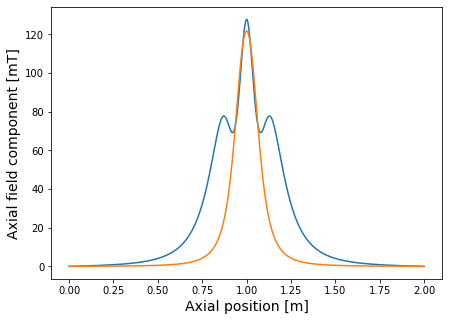
\includegraphics[width=0.7\textwidth]{two_fields}
    \caption{Field profiles \textquotedblleft compared\textquotedblright}
  \end{figure}
\end{frame}

\begin{frame}
  \frametitle{Beam state tracking - narrow}
  \begin{figure}
    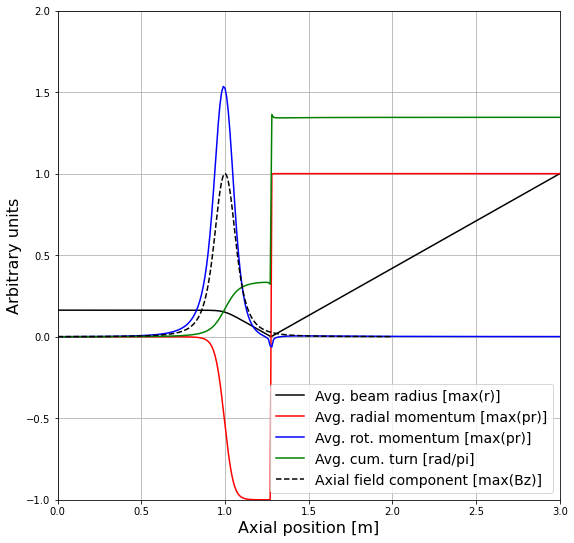
\includegraphics[width=0.8\textwidth]{felddurchgang_narrow}
  \end{figure}
\end{frame}

\begin{frame}
  \frametitle{Beam state tracking - wide}
  \begin{figure}
    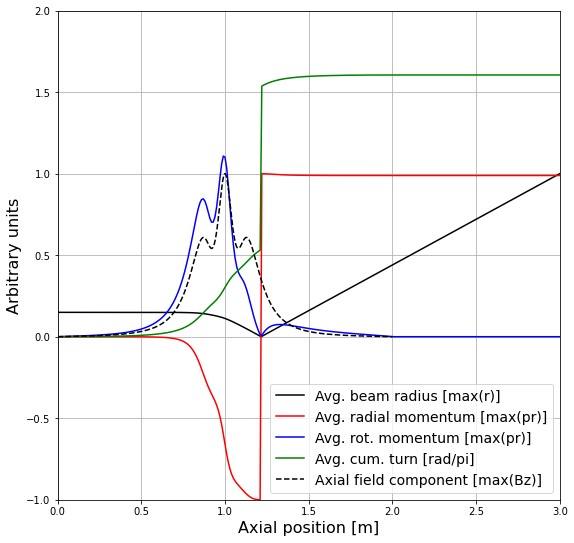
\includegraphics[width=0.8\textwidth]{felddurchgang_wide}
  \end{figure}
\end{frame}

\begin{frame}
  \frametitle{Focal region zoom - wide}
  \begin{figure}
    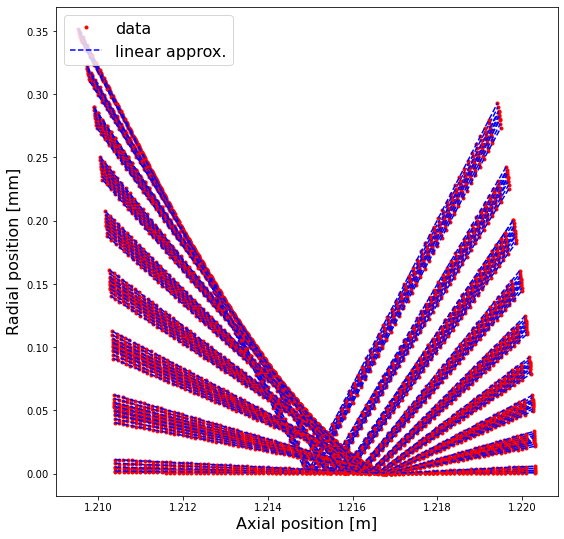
\includegraphics[width=0.8\textwidth]{focus_zoom_wide}
  \end{figure}
\end{frame}

\begin{frame}
  \frametitle{Focal region zoom - narrow}
  \begin{figure}
    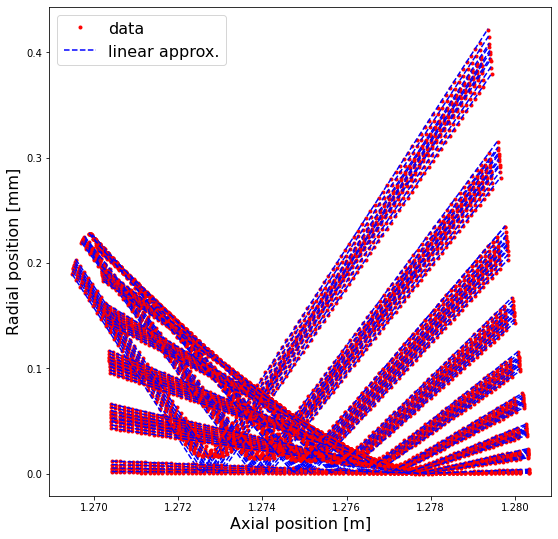
\includegraphics[width=0.8\textwidth]{focus_zoom_narrow}
  \end{figure}
\end{frame}

\begin{frame}
  \frametitle{Rotary momentum distribution}
  \begin{figure}
    \begin{tabular}{cc}
      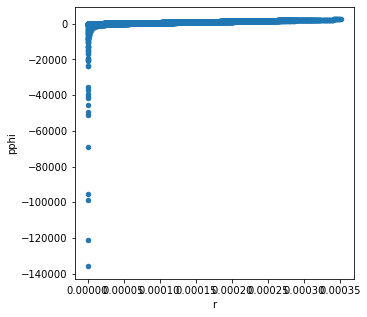
\includegraphics[width=0.5\textwidth]{r_pphi_wide} &
      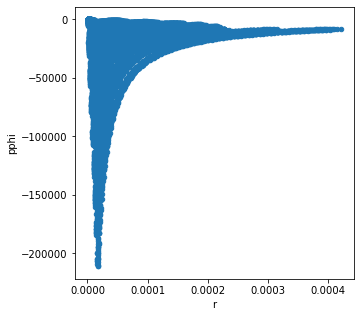
\includegraphics[width=0.5\textwidth]{r_pphi_narrow}
    \end{tabular}
  \end{figure}
\end{frame}

\begin{frame}
  \frametitle{Spherical aberrations - wide}
  \begin{figure}
    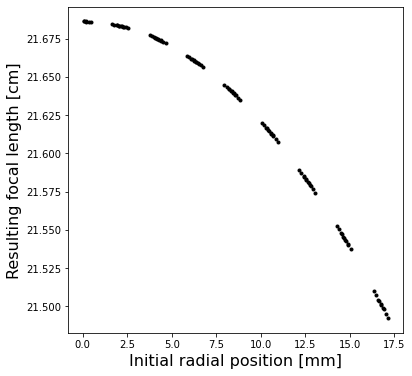
\includegraphics[width=0.8\textwidth]{andriis_field_foci}
  \end{figure}
\end{frame}

\begin{frame}
  \frametitle{Spherical aberrations - comparison}
  \begin{figure}
    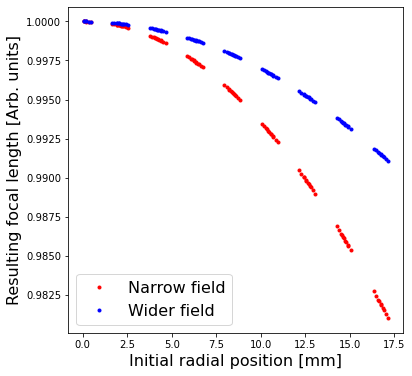
\includegraphics[width=0.8\textwidth]{foci_compare_two_fields}
  \end{figure}
\end{frame}

%\section{Section 2}
%\begin{frame}%
  %\frametitle{Title}
  %\framesubtitle{Subtitle}
%\end{frame}

%\section{Summary}
%\begin{frame}
%  \frametitle{Summary}
%  \framesubtitle{Subtitle}
%\end{frame}

%\begin{frame}[allowframebreaks]
%  \frametitle{References}
%  \printbibliography
%\end{frame}

\end{document}
